% under work, not implemented fully
\documentclass[landscape]{article}

\usepackage{siunitx}
\usepackage{tikz}
\usepackage{pgfplots}
\usepackage{drawproton}

\usetikzlibrary{calc}
\usetikzlibrary{fadings}
\usetikzlibrary{shadings}
\usetikzlibrary{shadows}
\usepgfplotslibrary{units}
\pgfplotsset{compat=newest,filter discard warning=false,tick scale binop=\times}

\tikzset{
 xq2shading/.style={
  rounded corners=5pt,
  drop shadow,
  preaction={
   fill=white,
   draw=black,
   line width=0.2pt
  },
  opacity=0.15,
  top color=red!70!magenta,
  bottom color=cyan,
  middle color=red!70!magenta!50!cyan!30!white,
  shading angle=45
 }
}
\pgfplotstableread{datafiles/pdfdataQ210.csv}\pdfdatatableA
\pgfplotstableread{datafiles/pdfdataQ2100.csv}\pdfdatatableB

\pagestyle{empty}

\begin{document}
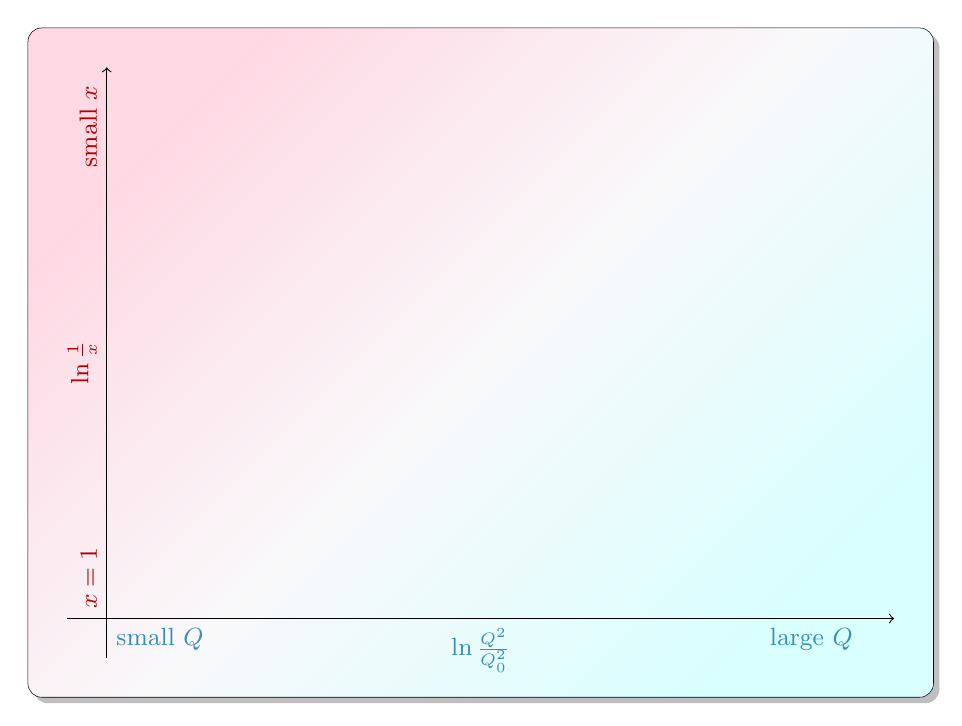
\begin{tikzpicture}
	\path[xq2shading] (-1.0,7.5) rectangle (10.5,-1.0);
	\draw[->,every node/.append style={above,red!70!black,rotate=90,font={\small}}] (0,-0.5) -- (0,7) node[at={(0,0)},above right] {$x=1$} node[pos=0.5] {$\ln\frac{1}{x}$} node[pos=0.9] {small $x$};
	\draw[->,every node/.append style={below,cyan!70!black,font={\small}}] (-0.5,0) -- (10,0) node[at={(0,0)},below right] {small $Q$} node[pos=0.5] {$\ln\frac{Q^2}{Q_0^2}$} node[pos=0.9] {large $Q$};

	\begin{scope}[scale=0.8,xshift=50pt,yshift=30pt]
		\foreach \iprotonx in {0,...,3} {
				% the parton evolution in x
				\foreach \iprotonq in {0,...,3} {
						\begin{scope}[xshift={90*\iprotonq *1pt},yshift={60*\iprotonx *1pt}]
							\pgfmathsetmacro{\partonlevel}{\iprotonx}
							\pgfmathsetmacro{\protonradius}{15 * (1 + 0.3 * sqrt(\iprotonx + 4*\iprotonq/3))}
							\drawproton[background=white,parton size decay rate={0},initial parton size={6-1.5*\iprotonq}]{\protonradius}{\partonlevel}{\partonlevel}
						\end{scope}
					}
			}
	\end{scope}
\end{tikzpicture}

\pagebreak

\begin{tikzpicture}
	\begin{scope}[yscale=0.4,xslant=0.6,every node/.append style={transform shape}]
		\path[xq2shading] (-1.0,7.5) rectangle (10.5,-1.0);
		\draw[->,every node/.append style={above,red!70!black,rotate=90,font={\small}}] (0,-0.5) -- (0,7) node[at={(0,0)},above right] {$x=1$} node[pos=0.5] {$\ln\frac{1}{x}$} node[pos=0.9] {small $x$};
		\draw[->,every node/.append style={below,cyan!70!black,font={\small}}] (-0.5,0) -- (10,0) node[at={(0,0)},below right] {small $Q$} node[pos=0.5] {$\ln\frac{Q^2}{Q_0^2}$} node[pos=0.9] {large $Q$};
		\node[red!70!black] at (5,7) {high energy collisions};
		\node[cyan!70!black,rotate=-90] at (10,3.5) {high momentum transfer};

		\begin{scope}[scale=0.8,xshift=50pt,yshift=30pt]
			\foreach \iprotonx in {0,...,3} {
					% the parton evolution in x
					\foreach \iprotonq in {0,...,3} {
							\begin{scope}[xshift={90*\iprotonq *1pt},yshift={60*\iprotonx *1pt}]
								\pgfmathsetmacro{\partonlevel}{\iprotonx}
								\pgfmathsetmacro{\protonradius}{15 * (1 + 0.3 * sqrt(\iprotonx + 4*\iprotonq/3))}
								\drawproton[background=white,parton size decay rate={0},initial parton size={6-1.5*\iprotonq}]{\protonradius}{\partonlevel}{\partonlevel}
								\coordinate (proton\iprotonx\iprotonq) at (0,0);
							\end{scope}
						}
				}
		\end{scope}
	\end{scope}
	\begin{scope}[
			yslant=0.66666666,scale=0.8,
			every axis/.append style={
					scale only axis=true,width=108pt,height=108pt,
					xmode=log,xmax=1,xmin=1e-4,ymin=1e-3,ymax=5,
					clip=false,
					axis background/.style={fill=white,fill opacity=0.7},
					x tick label style={opacity=0.5},
					x dir=reverse
				},
			overlay]
		\begin{axis}[legend to name={leg:pdflegend},legend columns=1,legend style={cells={anchor=mid west}},at={(proton01)}]
			\addplot[black,thick] table[x index=0,y index=2] {\pdfdatatableA}; % gluons
			\addplot[blue] table[x index=0,y index=3] {\pdfdatatableA}; % up
			\addplot[red] table[x index=0,y index=4] {\pdfdatatableA}; % down
			\addplot[orange] table[x index=0,y index=5] {\pdfdatatableA}; % upbar
			\addplot[green!50!black] table[x index=0,y index=6] {\pdfdatatableA}; % downbar

			\node[below left] at (rel axis cs:0.95,0.95) {\small$Q^2 = \SI{10}{GeV^2}$};
			\addlegendentry{gluon}
			\addlegendentry{up}
			\addlegendentry{down}
			\addlegendentry{antiup}
			\addlegendentry{antidown}
		\end{axis}
		\begin{axis}[at={(proton02)}]
			\addplot[black,thick,overlay] table[x index=0,y index=2] {\pdfdatatableB}; % gluons
			\addplot[blue] table[x index=0,y index=3] {\pdfdatatableB}; % up
			\addplot[red] table[x index=0,y index=4] {\pdfdatatableB}; % down
			\addplot[orange] table[x index=0,y index=5] {\pdfdatatableB}; % upbar
			\addplot[green!50!black] table[x index=0,y index=6] {\pdfdatatableB}; % downbar

			\node[below left] at (rel axis cs:0.95,0.95) {\small$Q^2 = \SI{100}{GeV^2}$};
		\end{axis}
	\end{scope}
	\path[scale=0.8] (proton01) +(0,108pt) node[above left,transform shape] {$xf(x,Q^2)$};
\end{tikzpicture}
\end{document}
